\chapter{Generating Normal Random Variables}

\setcounter{problem}{1}
\section{Discussion}

\begin{fullwidth}


The goal of this lab is to generate normal random variables but using the Central limit  theorem instead of the inverse transform or the accept reject method. The hard part about all of this is using the right variance and shifting from $N(0,1)$ to the general $N(\mu, \sigma^2)$. Use filename {\tt rnorm.py}.

\section{Steps}

\step First, let's define some constants and the variance of a uniform variable:

\begin{pyverbatim}
def varunif(a,b):
	return ((b-a)**2)/12.0
N = 20
MEAN = 0.0
VARIANCE = 2
TRIALS = 2000
\end{pyverbatim}

\step  We ultimately need to define some functions to generate random normal variables, but let's fill in the code we need to draw a histogram and then the theoretical distribution on top:

\begin{pyverbatim}
# Get X_ taken from TRIALS trials, plot histogram normalized to density func
X_ = [rnorm(MEAN,VARIANCE) for i in range(TRIALS)]
plt.hist(X_, normed=1)

# plot real normal curve
x = np.arange(min(X_),max(X_), 0.01)
y = stats.norm.pdf(x, MEAN, math.sqrt(VARIANCE))
plt.plot(x,y, color='red')
plt.show()
\end{pyverbatim}

\step And, now for the tricky part:  Define a function that returns a random variable from $N(0,1)$.

\begin{pyverbatim}
def rnorm_():
    "yield N(0,1) value"
    ...
\end{pyverbatim}	

To do this, get $N$ random uniform values from $U(0,1)$ into $X$. Then compute the mean, $\overline X$. Shift that value so that is 0-centered and call it $rv$. We know from theory that the variance of $\overline X$ is $\sigma^2 / N$, where $\sigma^2$ is the variance of the underlying distribution $U(0,1)$, but we need the variance to be 1. Scale $rv$ so that it has variance 1. Note that a ``standard normal'' variable can be created from an arbitrary normal $X$ via $Z = (X-\mu)/\sigma$.

\step Now define a more general method that lets us specify the mean and variance (not the mean and the standard deviation):

\begin{pyverbatim}
def rnorm(mean, variance):
    get a random variable from N(0,1) and shift mean then scale
\end{pyverbatim}	

From the standard normal variable we get from the previous function, we can use $X = \mu+ Z\sigma$.

\step Run it and you should get the following graph:

\scalebox{.35}{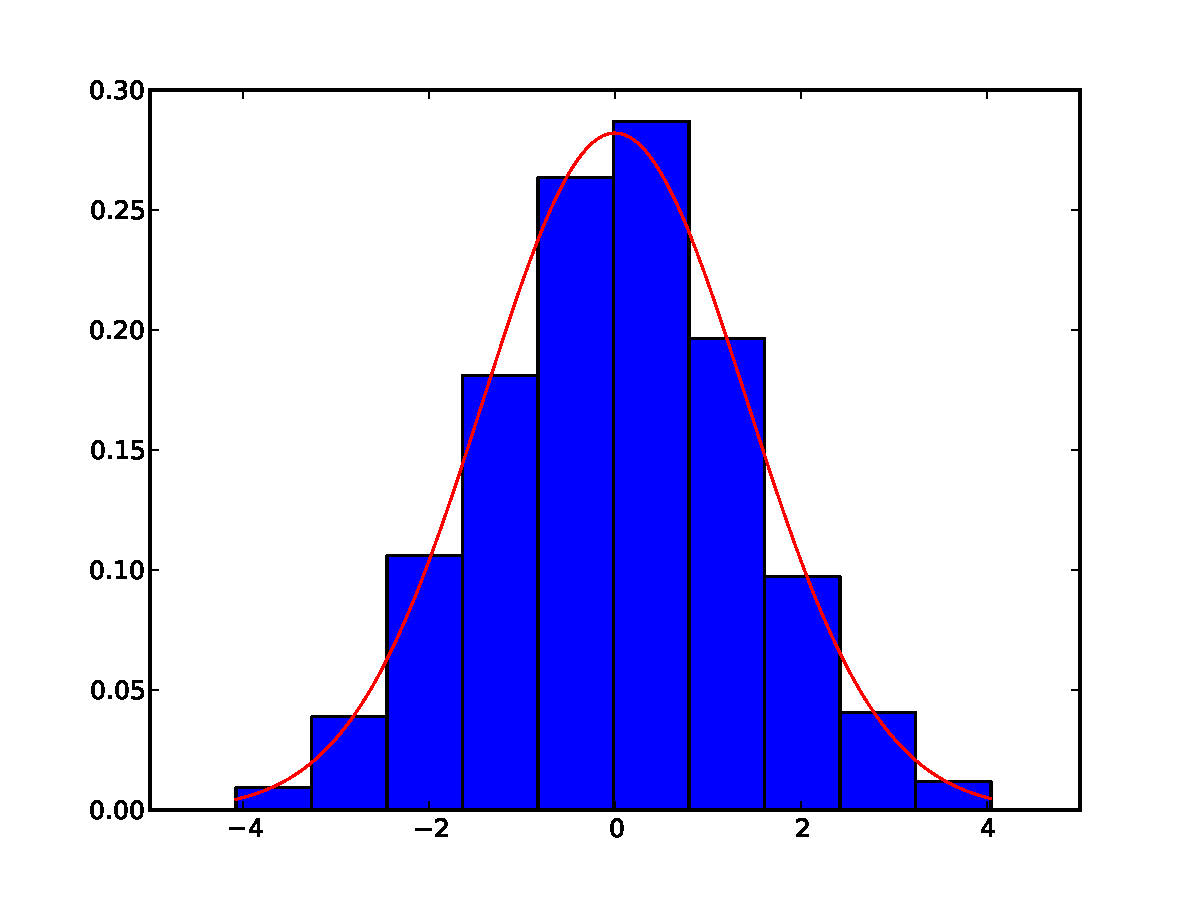
\includegraphics{figures/rnorm-2000-20.pdf}}

\section{Deliverables}

Please submit:

\begin{itemize}
\item your {\tt rnorm.py} file
\item a PDF of the graph shown above.
\end{itemize}

\end{fullwidth}

